\section{Schritt für Schritt Anleitung}
\label{sec:StepbyStep}
Eine Schritt für Schritt Anleitung zum vollständigen Scannen und exportieren eines 3D-Objektes.

\begin{longtable}{|>{\RaggedRight}m{5cm}|m{8cm}|} 
\caption{Schritt für Schritt Anleitung} 
\label{tab:StepbyStep}
\\ \hline
\multicolumn{2}{|c|}{\textbf{Schritt für Schritt Anleitung}}
\\ \hline 
\endfirsthead


\multicolumn{2}{|c|}%
{{ Fortsetzung }} 
\\ \hline 
%\multicolumn{1}{|c|}{\textbf{Time (s)}} &
%\multicolumn{1}{c|}{\textbf{Triple chosen}} 
%\\ \hline 
\endhead


\multicolumn{2}{|l|}%
{{\textbf{Schritt 1 - Starten von RapidForm2004}}}
\\ \hline
Auf dem Desktop doppelt auf das RapidForm Icon klicken.
& 
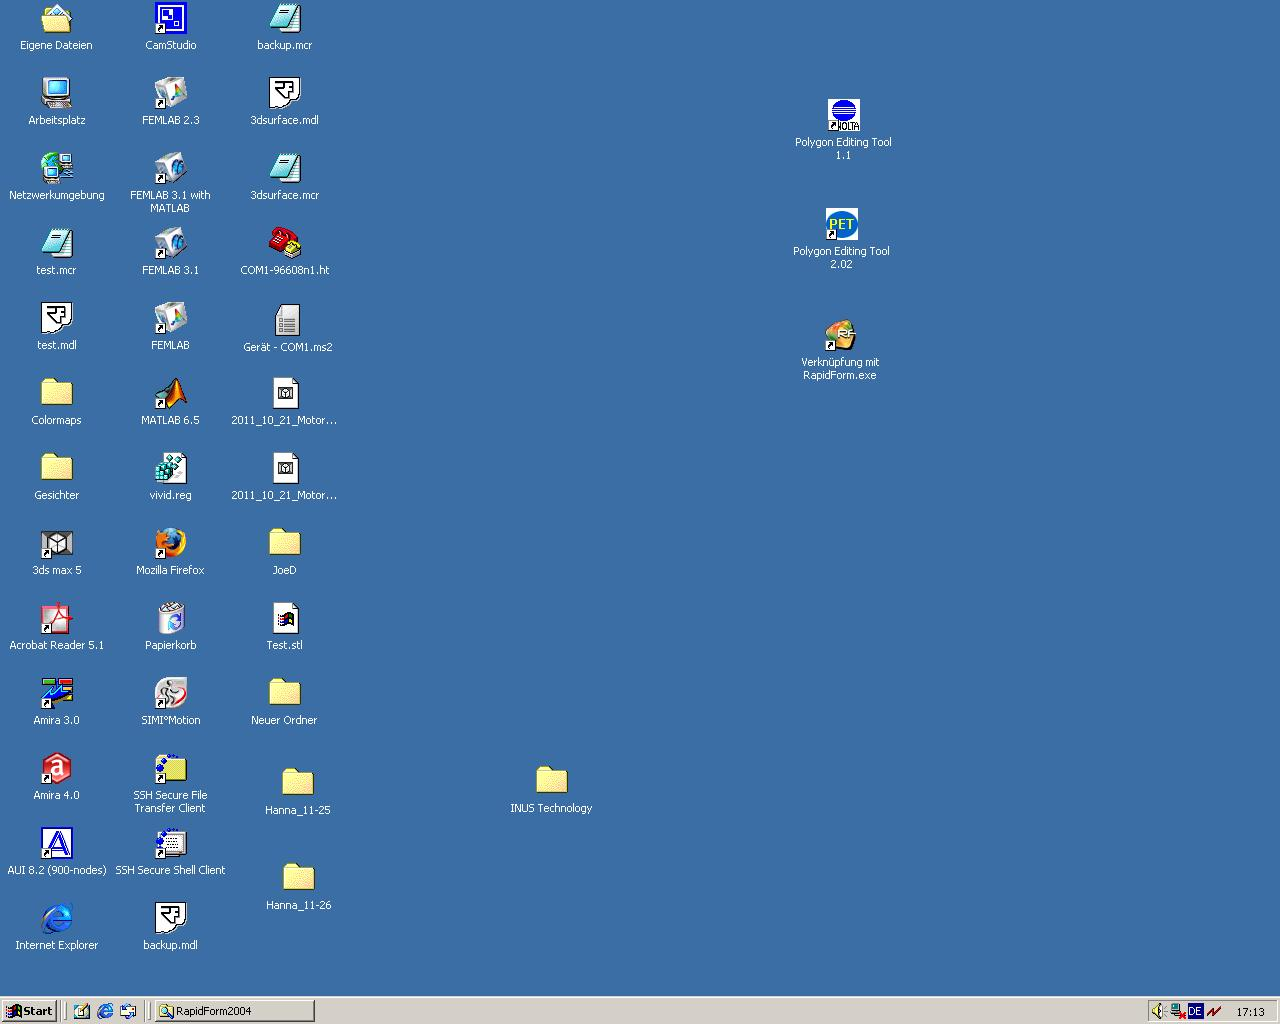
\includegraphics[width=8cm]{Anleitung/1_Desktop}
\\ \hline 
 
\multicolumn{2}{|l|}%
{{\textbf{Schritt 2 - Oberfläche von RapidForm2004}}}
\\ \hline
Die Oberfläche unterteilt sich in Menü, Werkzeugleisten, Projektbaum und ??.
Je nach dem welche Ansicht in ?? gewählt ist, verändern sich auch das Menü und die Werkzeugleisten. 
& 
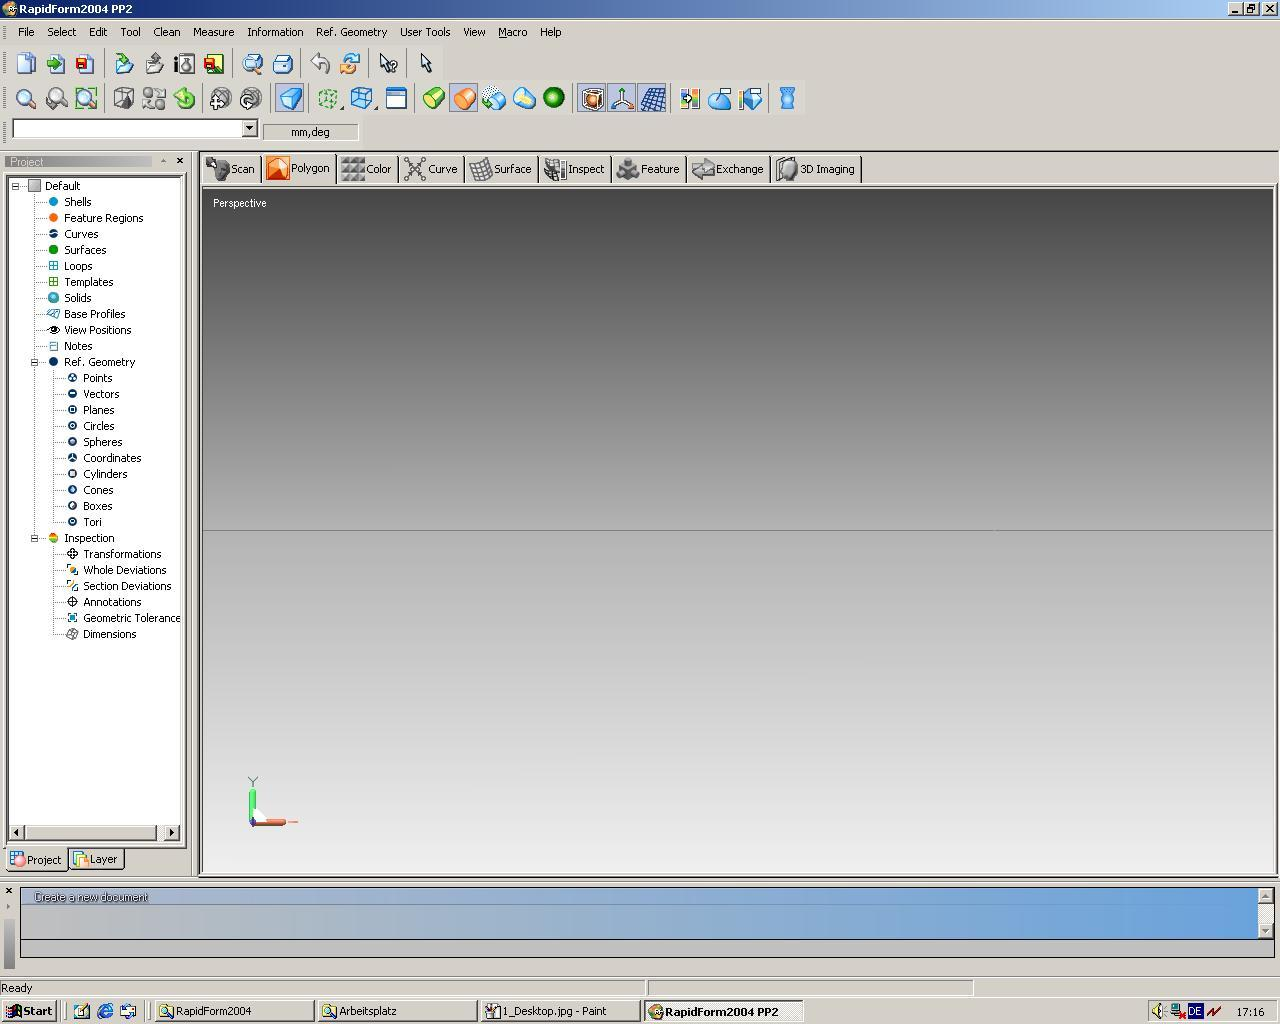
\includegraphics[width=8cm]{Anleitung/2_RapidForm}
\\ \hline  

\pagebreak 





\multicolumn{2}{|l|}%
{{\textbf{Schritt 3 - Starten des ''ADD-IN''}}}
\\ \hline
In der Menüzeile auf 
\textbf{Macro -> Addins -> Konica Minolta VIVID Direct Control Addin v2.6.11}
klicken.
& 
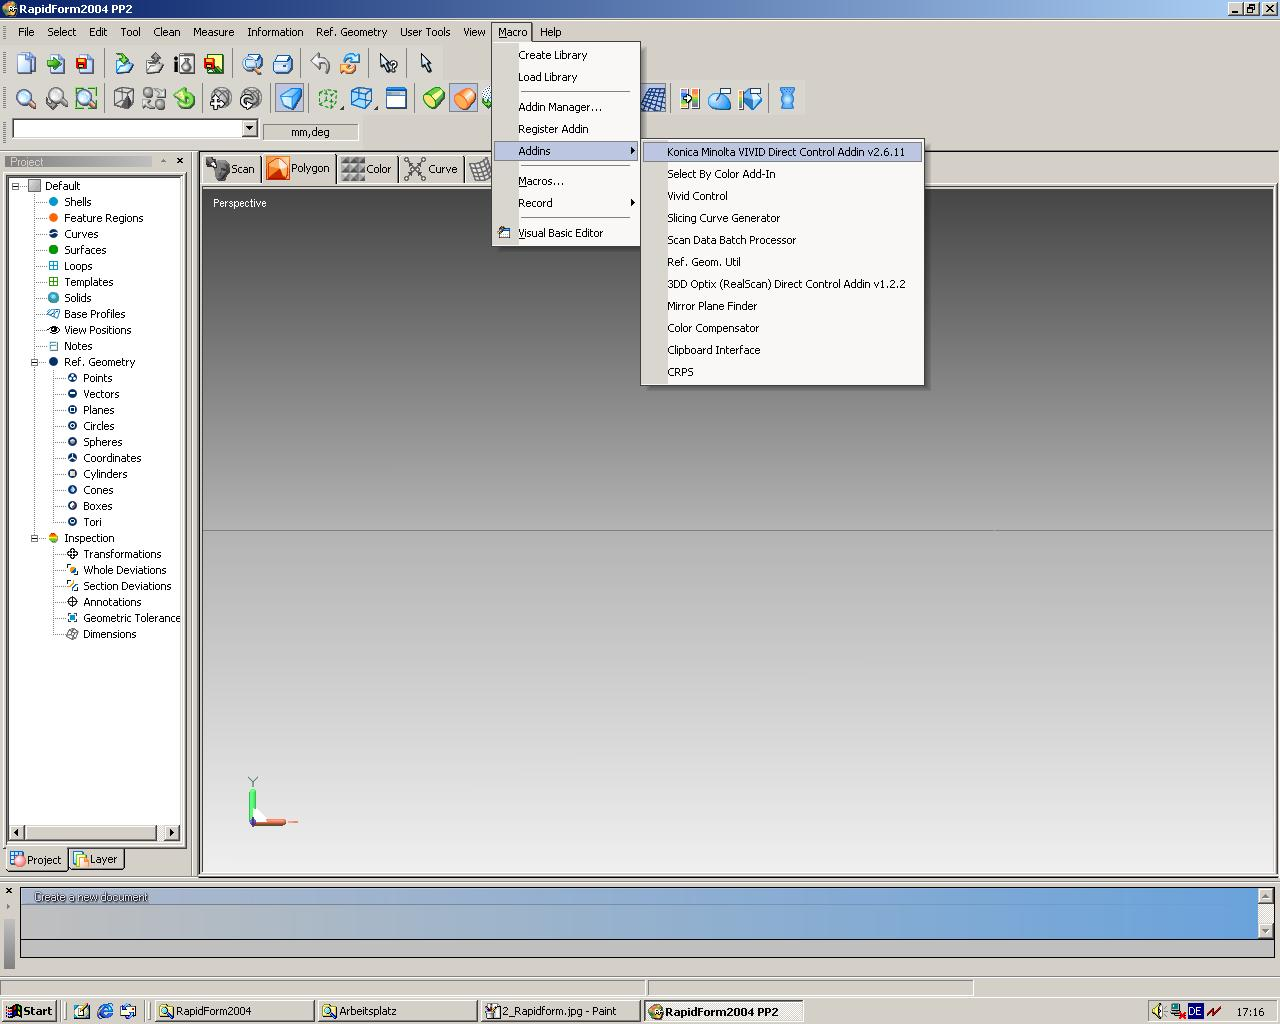
\includegraphics[width=8cm]{Anleitung/3_ADDIN_Menu}
\\ \hline  

\multicolumn{2}{|l|}%
{{\textbf{Schritt 4 - Kalibrieren vorbereiten}}}
\\ \hline
\begin{TippS}Für ein erfolgreiches Zusammenführen der einzelnen Aufnahmen ist die Kalibrierung unerlässlich!\end{TippS}
Auf dem Add-In Panel, unter dem Vorschau Fenster, auf \textbf{Live-Preview} klicken. \linebreak
Das Kalibrierungsblech auf dem Drehtisch positionieren.  \linebreak
Dabei muss der Noppen an der Unterseite des Kalibrierungsblechs in das mittlere Loch des Drehtisches gesteckt werden. Die abgeklebte Seite muss zum VI-900 zeigen.
& 
%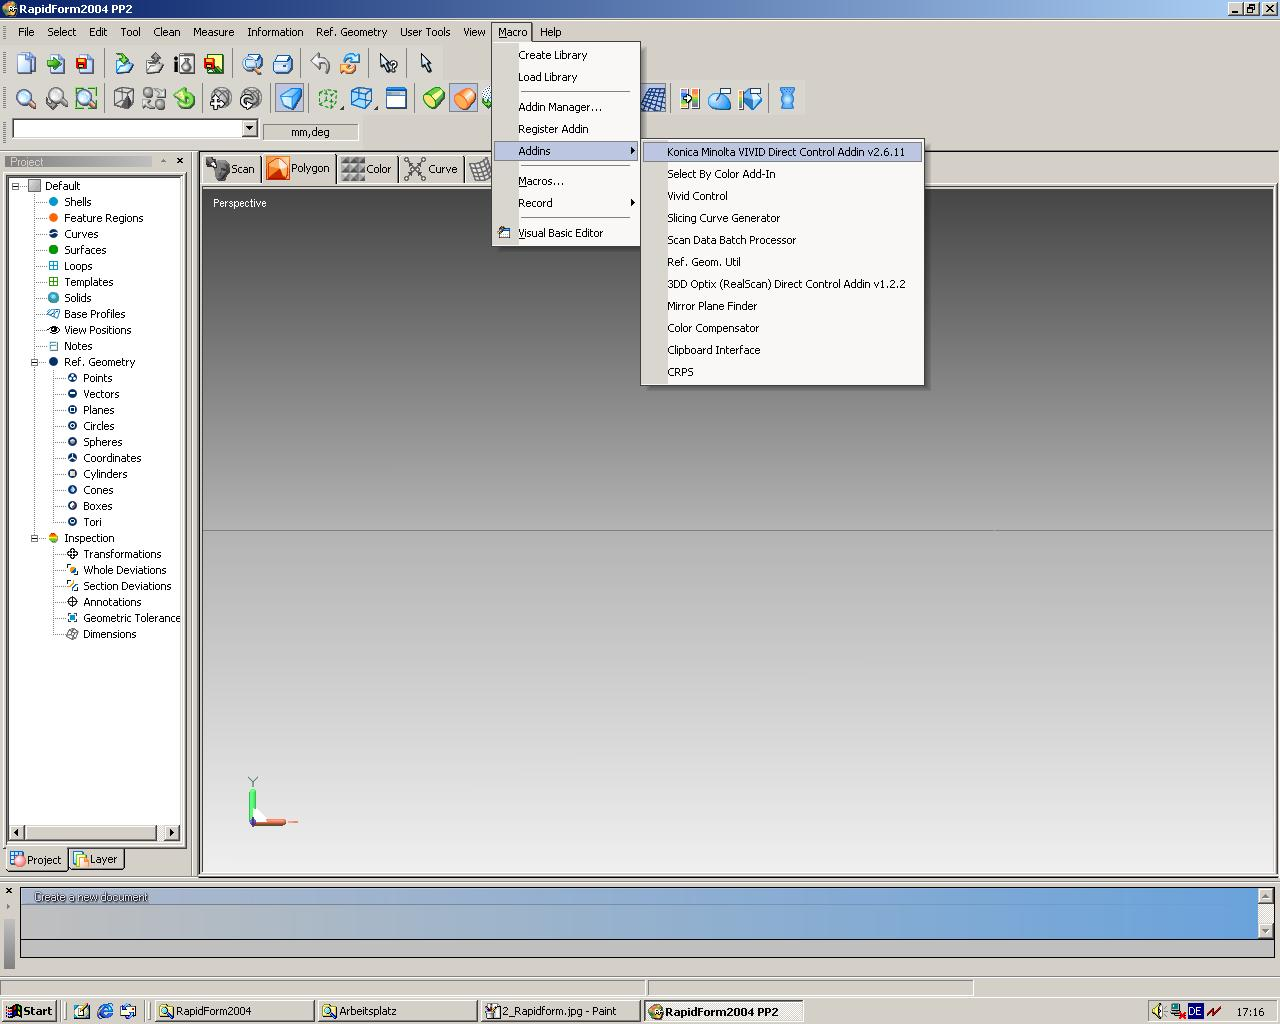
\includegraphics[width=8cm]{Anleitung/3_ADDIN_Menu}
Bild?
\\ \hline  

\pagebreak 



\multicolumn{2}{|l|}%
{{\textbf{Schritt 5 - Kalibrieren}}}
\\ \hline
Den Reiter \textbf{VIVID: 1} auswählen.\linebreak
Bei \textbf{Manual Para.} ein Häkchen setzen.\linebreak
Im Feld \textbf{Laser Power} ''23'' eintragen.\linebreak
Auf \textbf{Scan for Calib} klicken.
& 
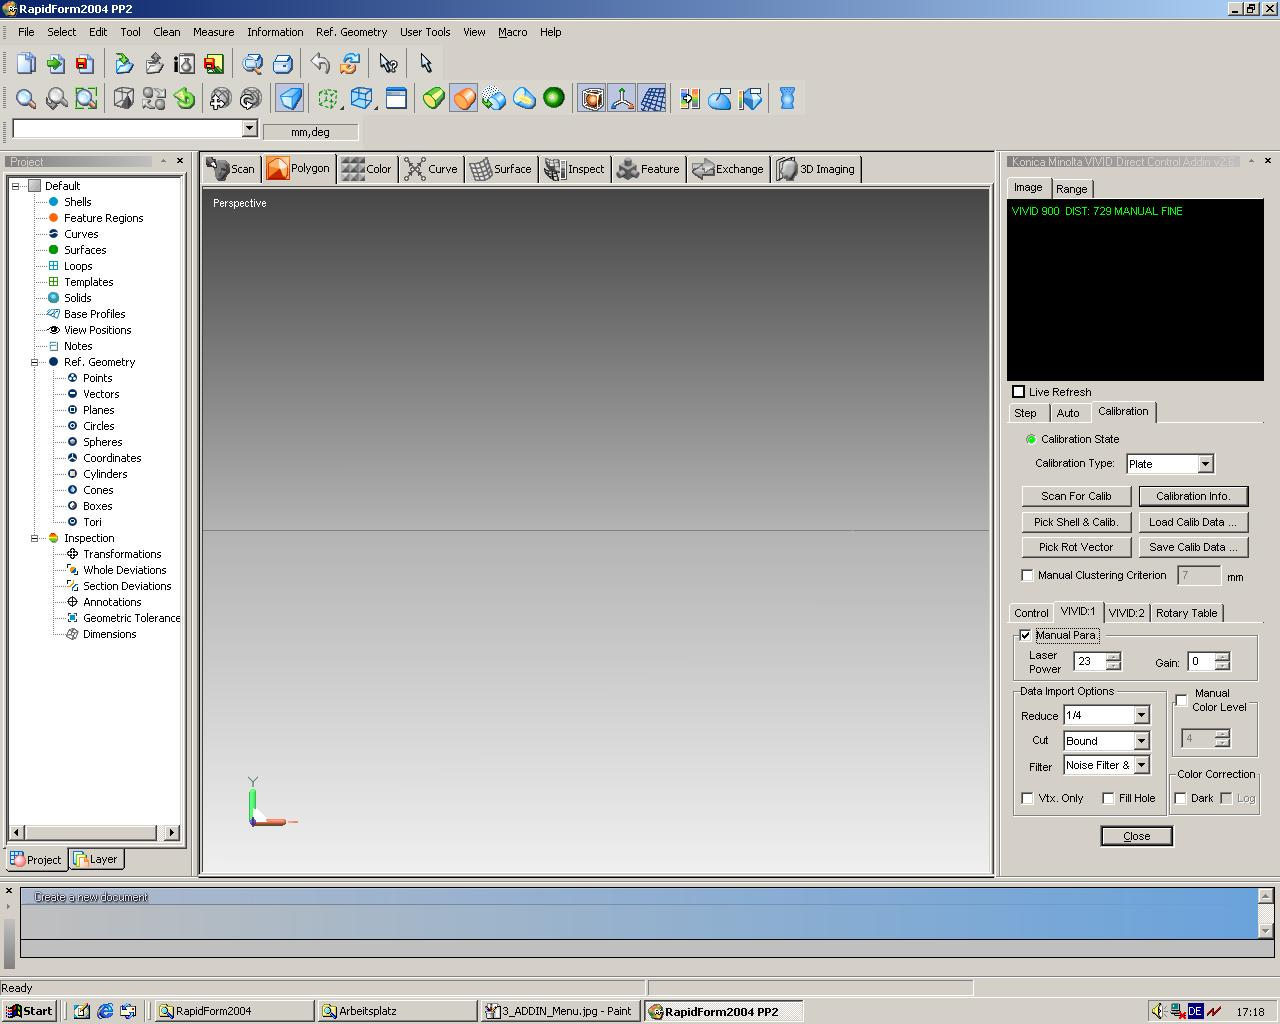
\includegraphics[width=8cm]{Anleitung/4_Calibration}
\\ \hline  

\multicolumn{2}{|l|}%
{{\textbf{Schritt 6 - Kalibrierungsergebnis}}}
\\ \hline
Das Ergebnis sollte ähnlich zu dem in der rechten Abbildung sein. \linebreak
Falls das Add-In einen Fehler ausgibt, muss das Kalibrierungsblech eventuell anders positioniert werden oder der Wert im Feld \textbf{Laser Power} verändert werden.
& 
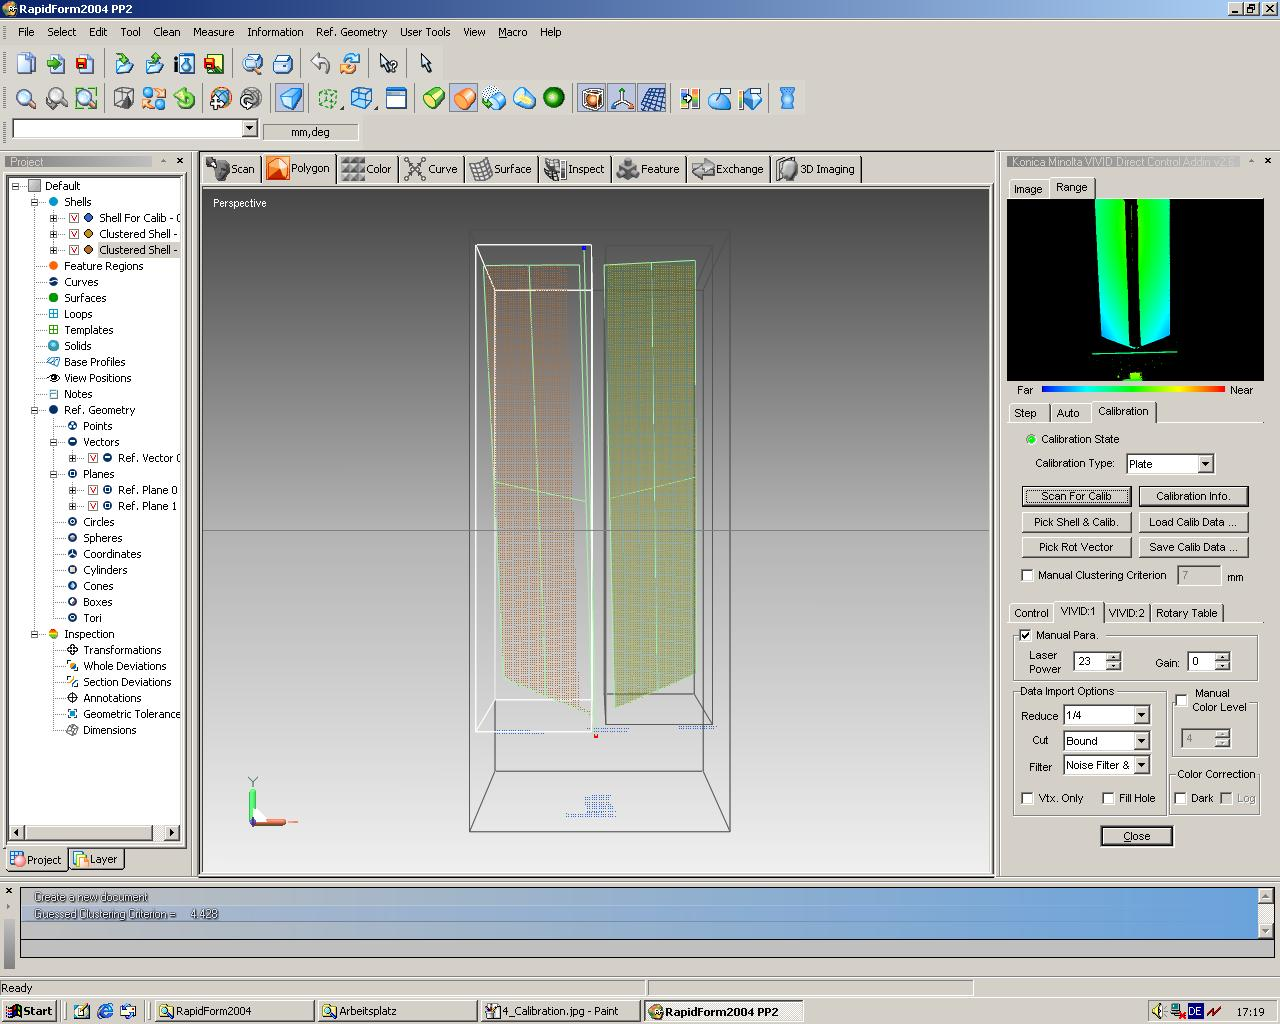
\includegraphics[width=8cm]{Anleitung/4_Calibration_result}
\\ \hline  

\pagebreak 



\multicolumn{2}{|l|}%
{{\textbf{Schritt 6 - Kalibrieren}}}
\\ \hline
Im neu geöffneten AddIn-Panel auf \textbf{Scan for Calib} klicken.

& 
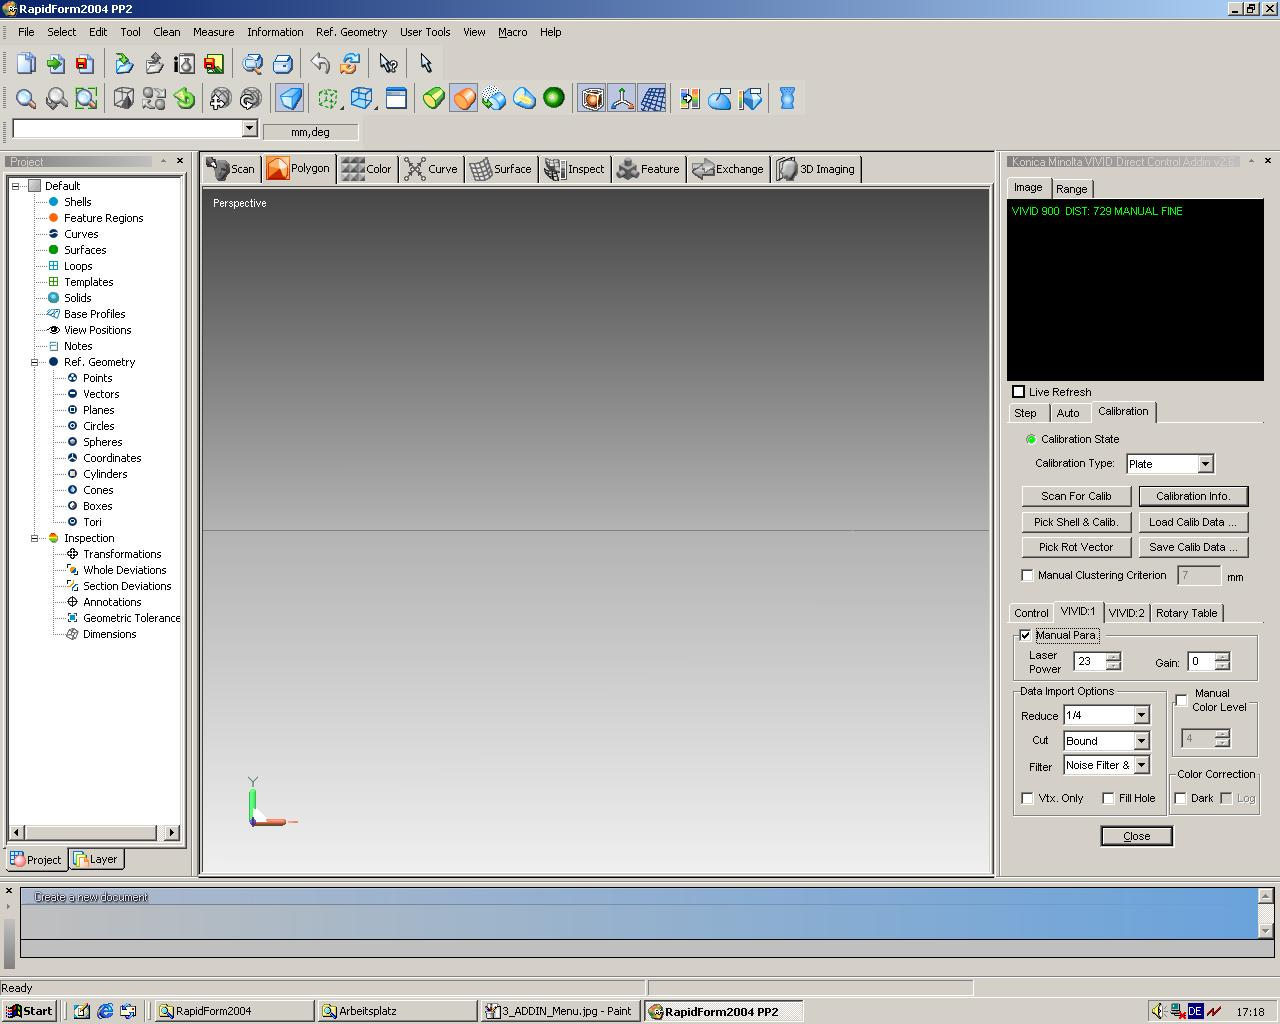
\includegraphics[width=8cm]{Anleitung/4_Calibration}
\\ \hline  
\pagebreak 





\end{longtable} 

